% Permission is granted to copy, distribute and/or modify this document
% under the terms of the GNU Free Documentation License, Version 1.3
% or any later version published by the Free Software Foundation;
% with no Invariant Sections, no Front-Cover Texts, and no Back-Cover Texts.
% A copy of the license is included in the section entitled "GNU
% Free Documentation License".
%
% Authors:
% Caner Candan <caner@candan.fr>, http://caner.candan.fr

\documentclass[twocolumn,oneside,10pt]{article}
\usepackage[french,url,algo]{my_package}

\title{{\bf Elevator}\\{\em Architecture des systèmes embarqués}}

\newcommand {\elevator}   {{\em Elevator}}

\begin{document}

\maketitle

%\tableofcontents
%\newpage

\begin{abstract}

Commençons par un rappel des objectifs attendus du rapport:\\

\begin{itemize}
\item présenter un graphe d'état illustrant tous les processus nécessaire au fonctionnement de l'ascenseur,
\item créer un simulateur d'ascenseur en langage C/C++.
\end{itemize}

\paragraph{\elevator}

Le projet est un simulateur d'ascenseur développé en C++. N'ayant pas eu le temps d'étudier une implémentation de ``SystemC'', un design a tout de même était élaboré afin de généraliser les différents composants que compte le projet. Le langage offrant des routines de généricité, il est ainsi possible d'interchanger certain processus. Ce qui rend le simulateur plus robuste.

\end{abstract}

\section{Graphe d'états}

De manière générale, le diagramme d'états définit l'ensemble des états couvert par un système quelconque. Les paramètres, du système, peuvent être modifiés lors d'un changement d'état. Nous présentons le graphe d'état du simulateur \elevator\ en figure \ref{fig:graphe_etat}.

\begin{figure}[h]
  \centering
  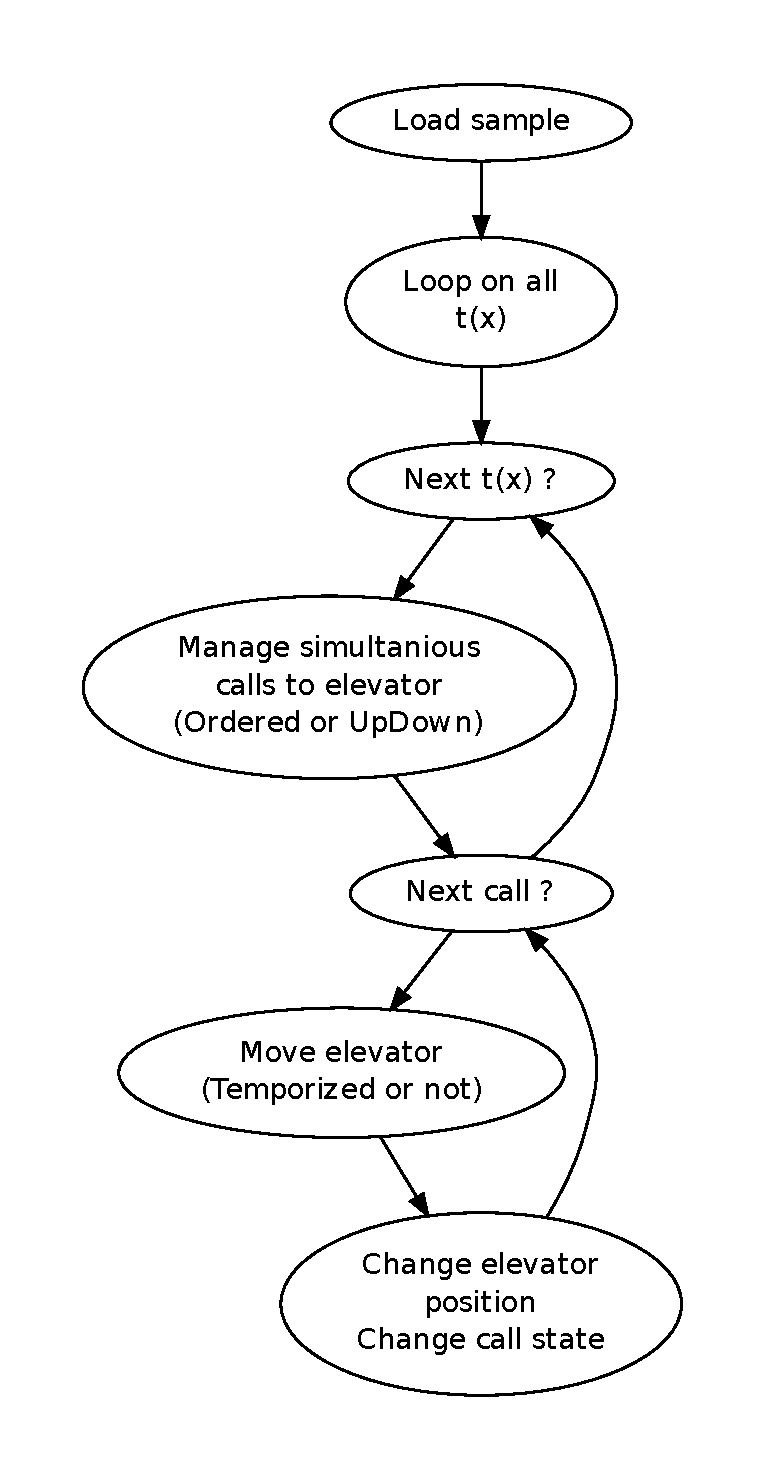
\includegraphics[scale=0.50]{images/elevator}
  \caption{Graphe d'états}
  \label{fig:graphe_etat}
\end{figure}

\section{Les composants}

Comme nous le disions, le simulateur \elevator\ est doté d'un design intuitif. On peut ainsi distinguer plusieurs familles de composants au sein du projet. Ci-dessous une liste non-exhaustive de composants détaillés.

\paragraph{\em Elevator}

Ce composant représente l'ascenseur en lui même. Il est possible d'intégrer plusieurs types d'ascenseurs en partant des plus simples aux plus complexes. Ci-dessous la liste des ascenseurs.\\

\begin{itemize}
\item {\em EasyElevator}, un simple ascenseur. Il se limite à l'enregistrement de sa position.\\
\item {\em OpenCloseElevator}, une variante doté d'une porte à ouvrir et fermer.
\end{itemize}

\paragraph{\em Move}

Ce composant gére les appels simultannés à l'ascenseur puis délégue son déplacement vers une autre famille de composant {\em OneMove}. Ci-dessous une liste de ses composants.\\

\begin{itemize}
\item {\em OrderedMove}, ce gestionnaire de mouvement effectue les déplacements à travers les étages demandés de manière ordonnée.\\
\item {\em UpDownMove}, une variante effectuant des déplacements, en premier lieu, vers le haut puis vers le bas. Il est possible de produire l'inverse.
\end{itemize}

\paragraph{\em OneMove}

Ce composant effectue le déplacement d'un étage initial vers un étage cible. Ci-dessous la liste des ses composants.\\

\begin{itemize}
\item {\em DummyOneMove}, un simple déplaceur d'ascenseur.\\
\item {\em TemporizedOneMove}, une variante qui calcule la distance entre l'étage de départ et d'arrivée et temporise le déplacement. Il est possible de définir le temps de déplacement nécessaire par pas d'étage.
\end{itemize}

\paragraph{\em ScheduleSampler}

Ce composant permet la lecture d'un fichier contenant le scénario à jouer par le simulateur. Nous présentons dans le code \ref{sample_example} un exemple d'échantillon.

\begin{algorithm}[h]
  \caption{Exemple de fichier de scénario executable par le simulateur \elevator}
  \label{sample_example}
\begin{verbatim}
0 10 20 -50
-70 0 0 0 0
-9
-8
-7
-6 -5 -4 -3 -2 -1
\end{verbatim}
\end{algorithm}

Chaque ligne du fichier représente un temps $t$ et à chaque temps $t$ il est possible de faire des appels simultanés à l'ascenseur.

\paragraph{\em Scheduler}

Il existe une composante principale du simulateur, il s'agit du {\em Scheduler} qui utilise l'ensemble des composants cités précédement à travers un jeu de paramètrage, y compris le scénario à jouer, et lance la simulation. Ci-dessous la liste de ses composants.\\

\begin{itemize}
\item {\em LoopScheduler}, juste une variante executant le scénario en boucle.
\end{itemize}

\section{L'assemblage}

L'assemble consiste à regrouper les différents composants présentés et former le simulateur souhaité.

\paragraph{Exemple d'assemblage des composants}

Le code \ref{exemple_simulateur} donne un exemple d'assemblage des composants pour former le simulateur.

\begin{algorithm}[h]
  \caption{Exemple de code du simulateur assemblant différents types de composants}
  \label{exemple_simulateur}
\begin{verbatim}
int main(void)
{
  ScheduleSampler sampler("hard1.sdl");
  EasyElevator elevator;
  TemporizedOneMove onemove;
  UpDownMove move(elevator, onemove);
  Scheduler scheduler(move);
  scheduler(sampler());
}
\end{verbatim}
\end{algorithm}

Ce code illustre l'utilisation par le simulateur d'un échantillon de scénario ``hard1.sdl''\footnote{Présenté dans le code \ref{sample_example}}, d'un ascenseur simple, d'une temporisation des déplacements de l'ascenseur, d'un gestionnaire de déplacement privilégiant les déplacements vers le haut puis vers le bas puis finalement d'une execution du scénario.

\paragraph{Par défaut}

Certains paramètres ne sont pas définit dans le code, ils restent toutefois définit avec des valeurs par défaut, comme le pas de temps de déplacement du composant {\em TemporizedOneMove} qui est définit par défaut à 1 seconde. De même pour la position initiale de l'ascenseur définit à l'étage 0 par défaut.

\section{L'exécution}

Le code \ref{exemple_execution} illustre des résultats d'exécution obtenus avec le même échantillon présenté dans le code \ref{sample_example}.

\begin{algorithm}[h]
  \caption{Résultats obtenus après une execution du simulateur}
  \label{exemple_execution}
\begin{verbatim}
$> ./elevator samples/hard1.sdl
///// Scheduling /////
t(0) = -50 0 10 20
t(1) = -70 0
t(2) = -9
t(3) = -8
t(4) = -7
t(5) = -6 -5 -4 -3 -2 -1
//////////////////////

upper asked levels: .......... 10 ........
.. 20
lower asked levels: .................... 0
..........................................
........ -50
upper asked levels: ......................
............................ 0
lower asked levels: ......................
..........................................
...... -70
upper asked levels: ......................
....................................... -9
lower asked levels:
upper asked levels: . -8
lower asked levels:
upper asked levels: . -7
lower asked levels:
upper asked levels: . -6 . -5 . -4 . -3 .
-2 . -1
lower asked levels:
\end{verbatim}
\end{algorithm}

Sur les premières lignes des résultats, apparait un rappel du scénario qui va être joué par le simulateur \elevator, chaque ligne représentant une unité de temps $t$. Commence alors la simulation. Comme nous utilisons le composant {\em UpDownMove}, nous pouvons confirmer, par les résultats, que la simulation commence à parcourir les étages supérieurs demandés. Puis après avoir parcourut tous les étages supérieurs, le simulateur s'attaque aux étages inférieurs. Les points intermédiaires entre étage sont générés par le composant {\em TemporizedOneMove} pour indiquer les coûts en pas de temps entre deux étages.

\section{Conclusion}

Le simulateur \elevator\ a été conçu de manière à s'abstraire des specifications du système. Un langage plus approprié, comme ``SystemC'', aurait surement apporté un modèle plus optimal. Toutefois nous avons vu, à travers le design, qu'il est possible, en ayant une approche composant, d'interchanger les différents processus de notre système.\\

Ainsi libre à chacun de concevoir de nouveaux composants pour enrichir le simulateur avec de nouvelles fonctionnalités. L'ensemble du code du simulateur n'étant pas toute à fait générique, il reste des zones dans le code que l'on peut encore abstraire.\\

Ce papier suit les termes de la licence ``GNU Free Documentation License 1.3'' et peut être librement téléchargé\footnote{https://github.com/canercandan/elevator}, utilisé et modifié.

\end{document}
